\documentclass[11pt,twoside,a4paper]{book}
\usepackage[shorthands=off,english]{babel} % package for multilingual support

\RequirePackage{iftex}
\ifPDFTeX
    \usepackage[utf8]{inputenc}
    \usepackage[T1]{fontenc}
    % \usepackage{lmodern}
\else
    \RequirePackage{fontspec} % UFT8 fonts for LuaLaTeX
    % \setmainfont{Latin Modern Roman}
\fi
\usepackage{csquotes}

\usepackage[ backend=biber
            , style=numeric
            , sortlocale=en_US
            , bibencoding=UTF8
            , maxcitenames=3
            , maxbibnames=100
            ]{biblatex}

\usepackage{xcolor}
\definecolor{dark-red}{rgb}{0.6,0.15,0.15}
\definecolor{dark-green}{rgb}{0.15,0.4,0.15}
\definecolor{medium-blue}{rgb}{0,0,0.5}
\definecolor{paradisegreen}{HTML}{45A931}

\usepackage{amssymb,amsmath}
\usepackage{minted}
\usepackage{verbatim}
\usepackage[final]{listings}
\lstset{ language=C++ }
\usepackage{paralist}
% use upquote for straight quotes in verbatim environments
\usepackage{upquote}
\usepackage{booktabs}

\usepackage{xspace}
\usepackage{pgf}
\usepackage{tikz}
\usetikzlibrary{shapes, arrows, shadows, positioning, calc, fit, backgrounds, decorations.pathmorphing, automata, matrix}

\usepackage{pdfpages}

\usepackage{float}
\makeatletter
% custom float style, derived from ruled
% - caption is at the bottom
% - spaces before and after figure are larger
% - rules are thinner
% - bottom rule is missing
\newcommand\floatc@botruled[2]{{\@fs@cfont #1} #2\par}
\newcommand\fs@botruled{\def\@fs@cfont{\bfseries}\let\@fs@capt\floatc@botruled
    \def\@fs@pre{\hrule\kern0.5\abovecaptionskip}%
    \def\@fs@post{}%
    \def\@fs@mid{\kern0.5\abovecaptionskip\hrule\kern0.5\abovecaptionskip}%
\let\@fs@iftopcapt\iffalse}
\makeatother
\floatstyle{botruled}
\restylefloat{figure}
% \restylefloat{table}
\usepackage[labelfont=bf]{caption}

\usepackage{multirow}
\usepackage{microtype}

\usepackage{tabularx}
%\newcolumntype{C}{>{\centering\arraybackslash}X}
%\usepackage{arydshln}
\newcommand{\dg}{\textsuperscript{\dag}}

\usepackage{graphicx}
\usepackage{listings}
\usepackage{xspace}
\usepackage{bm}
\usepackage{rotating}
\usepackage{pbox}
\usepackage{pdflscape}
\usepackage{tabu, longtable}
\usepackage{array}
\usepackage{siunitx}
\usepackage{dsfont}
\usepackage{bytefield}

\usepackage{silence}

\newcommand{\mcrot}[4]{\multicolumn{#1}{#2}{\rlap{\rotatebox{#3}{#4}~}}}
\newcolumntype{L}[1]{>{\raggedright\let\newline\\\arraybackslash\hspace{0pt}}m{#1}}
\newcolumntype{C}[1]{>{\centering\let\newline\\\arraybackslash\hspace{0pt}}m{#1}}
\newcolumntype{R}[1]{>{\raggedleft\let\newline\\\arraybackslash\hspace{0pt}}m{#1}}
\newcommand\bithead[2]{\bitbox[]{#1}{\scriptsize #2}}


\newcommand\todo[1]{\noindent\textcolor{red}{(#1)}}
\newcommand\add[1]{\noindent\textcolor{green}{#1}}

\newcommand\tablecaption{Nothing}
\newcommand\tablecaptioncont{Nothing}
\newcommand\tablelabel{tab:todo}

\newcommand{\paradise}{ParaDiSe\xspace}

\newcommand{\FI}{Faculty of Informatics}
\newcommand{\MU}{Masaryk University}

\newcommand{\Jirik}{prof. RNDr. Jiří Barnat, Ph.D.}

\newcommand{\thesistitle}{RoFI -- Distributed Metamorphic Robots}
\newcommand{\thesissubtitle}{Masters's thesis}
\newcommand{\thesisauthor}{Jan Mrázek}
\newcommand{\thesisYearCity}{Brno, 2018}
\newcommand{\thesisadvisor}{\Jirik}

\newcommand{\note}{\textit{Note:}\xspace}

\newcommand{\fieldl}[1]{\multicolumn{2}{|c}{#1}}
\newcommand{\fieldr}[1]{\multicolumn{2}{|c|}{#1}}

\addbibresource{bibliography.bib}

% widdow and club fix
\clubpenalty 10000
\widowpenalty 10000

\usepackage{setspace}
\usepackage{placeins}

\addtolength\textwidth{5pt}
\addtolength\oddsidemargin{1cm}
\addtolength\evensidemargin{-1cm}

\usepackage[inline]{enumitem}
\providecommand{\tightlist}{%
    \setlength{\itemsep}{0pt}%
    \setlength{\parskip}{0pt}%
    \setlength{\topsep}{0pt}%
    \setlength{\partopsep}{0pt}}

\usepackage[ pdfauthor={Jan Mrázek}
            , pdftitle={RoFI -- Distributed Metamorphic Robots},
            , pdfsubject={Master's Thesis},
            , plainpages=false
            , pdfpagelabels
            , unicode
            , draft=false
            , colorlinks=true
            , linkcolor={dark-red}
            , citecolor={dark-green}
            , urlcolor={medium-blue}
            , unicode=true
            ]{hyperref}

% \newcommand{\TODO}[1]{\textbf{\color{red}#1}}

% autoref names
\addto\extrasenglish{
    \renewcommand{\chapterautorefname}{Chapter}
    \renewcommand{\sectionautorefname}{Section}
    \renewcommand{\subsectionautorefname}{Section}
}

\newcommand{\rot}[1]{\rotatebox{90}{#1\hspace*{0.5em}}}

\newcommand{\antispaceatend}{\vspace*{-\topsep}}

% \setlength{\overfullrule}{5pt} % TODO: remove

\begin{document}

% \DocLength{evensidemargin}
% \DocLength{oddsidemargin}
% \layout

% initial pages from Mornfall + modifications

\frontmatter
\pagestyle{empty}

\begin{center}
    {\Large \sc \FI, \MU}
    \vskip4em
    \includegraphics[width = 4cm, height = 4cm] {logo_fi.pdf}
    \vskip4em
    {\begin{spacing}{1}
        \Huge \bf \thesistitle
    \end{spacing}}
    \vskip2em
    {\Large \sc \thesissubtitle}
    \vskip4em
    {\LARGE \bf \thesisauthor}
    \vfill
    {\hfill \large \thesisYearCity}
\end{center}

\cleardoublepage

% only in print version!
\iffalse %@ifprint
\includepdf[pages={1}]{zadani.pdf}
\includepdf[pages={1}]{prohlaseni.pdf}
\cleardoublepage
\fi

\section*{Declaration} % from Mornfall
Thereby I declare that this thesis is my original work, which I have
created on my own. All sources and literature used in writing the
thesis, as well as any quoted material, are properly cited, including
full reference to its source.

\vfill
\textbf{Advisor:} \thesisadvisor

\cleardoublepage

\section*{Abstract}

TBA

\section*{Keywords}
TBA

\cleardoublepage

\section*{Acknowledgements}
First, I would like to thank all the people in the ParaDiSe laboratory for
providing such a nice half work-friendly and half procrastination-friendly
environment. It was a pleasure to write this thesis with you! Namely, I would
like to thank Jiří Barnat for providing me the opportunity to become a member of
ParaDiSe laboratory and advising this thesis, and Vladimír Štill for the instant
small consultations he provided me all the time.

I would like to thank Zuzana Baranová and Jana Mrázová for consulting the traps
of the English language with me. Also, I would like to thank my family for
supporting me and having enough patience with me.

Finally, I cannot forget to thank all the people who constantly reminded me to
work. This thesis would not exist without you.


\cleardoublepage
\thispagestyle{empty}

\pagestyle{headings}
\tableofcontents
\mainmatter

\chapter{Introduction}\label{chap:introduction}

There are many applications of robotic systems in today's world. The robotic
field has made enormous progress over the past decade, and robots can perform
various challenging tasks. However, the vast majority of robotic systems we can
find today is crafted for a given task and lacks versatility. For many
applications being single-task oriented is an advantage due to the simplicity
and efficiency of such a solution. However, for tasks like rescue missions,
space assemblies or new planet colonization versatility of robotic systems can
be a~crucial feature.

In the past decade, researches have been exploring \emph{modular robotic
systems}. These systems are assembled of modules. By reassembling the modules, a
new system with different capabilities is formed. This property makes such
systems versatile and allows them to perform tasks which cannot be tested in
advance (planet colonization) or tasks which feature unpredictable events
(rescue missions).

Research in this area runs in two parallel branches -- on one hand, there are
publications dealing with hardware design of the modules, on the other hand,
there are publications dealing with the algorithms for control synthesis and
reconfiguration of the systems. However, an interconnection of these two
research branches occurs only spuriously. We guess this is due to two factors:
\begin{enumerate*}
    \item the hardware publications often lack proper documentation as it is
    usually confidential and there is no possibility to get physical modules for
    verification of algorithms.
    \item The algorithmic publications often omit details of the physical
    limitations of the modules.
\end{enumerate*}

Therefore, in this thesis, we aim for an ambitious goal -- to introduce a new
modular robotic platform, the \emph{RoFI} platform, specially designed to
overcome the gap between algorithms and the physical world\footnote{We are aware
of the potential introduction of a new dead platform as nicely illustrated at
\url{https://xkcd.com/927/}.}. We target mainly at providing a full
specification of the platform with all its features at the expense of not
dealing with all technical aspects of the individual modules.

The thesis is structured as follows; the rest of this chapter gives an overview
of the modular robotic systems. In chapter \ref{chap:rofi} we define the RoFI
platform, in chapter \ref{chap:universal_module} we introduce the basic module
of the platform -- \emph{the universal module}, and in chapter
\ref{chap:software} we present software framework designed for the RoFI
platform. These chapters present the RoFI platform. Chapter
\ref{chap:prototypes} presents the current progress in a prototype
implementation of the universal module.

\section{Modular Robots}

A modular robotic platform is a way to build robots consisting of
\emph{modules}, as the name suggests. For our purposes, we consider a module to
be a single unit following a specification given by the platform. Modules are
rather high-level pieces with a certain level of self-control instead of
low-level components like individual actuators or sensors. It might even make
sense to talk about modules as individual robots, which are used to build other
robots \cite{brunete_current_2017}.

Each of these modules has a given set of capabilities. By joining multiple
modules and via their cooperation, new capabilities can emerge. Different
configurations of modules give rise to different capabilities. The modules are
usually mechanically connected to form a single robot.

The mechanical connection of the modules can be done externally, e.g., by an
operator, or can be performed by the modules on their own. In qte latter case,
we talk about \emph{self-reconfigurable} modules \cite{brunete_current_2017}.
Depending on the topology of the connection, there is a naming established in
the literature \cite{brunete_current_2017}:
\begin{enumerate*}
    \item \emph{chain type} for a linear, snake-like and tree-like
    configurations,
    \item \emph{lattice type} for regular grid-based robots,
    \item \emph{hybrid type} for robots combining both of previous approaches.
\end{enumerate*}
Further, if there is only a single or a few types of modules in the system, the
system is called \emph{metamorphic} \cite{brunete_current_2017}. Modules of such
a system are also called \emph{cells} as they mimic cells in living organisms.

The system can be \emph{centrally controlled} by a single (and possibly
external) unit, or the distributed nature of the modules can be leveraged, and
therefore, the system can feature \emph{distributed control}. The centrally
controlled approach is considered as an easier one; however, it does not utilize
all the potential computational power of the modules and it is harder to make
the system fault-tolerant (due to the presence of a single point of failure in
the form of the control unit) compared to the distributed control.

To build an intuition about the modular robots we give an analogy with
Replicators -- robots present in a sci-fi TV series Stargate
SG-1 \cite{wright_stargate_1997}. Readers unfamiliar with the TV series can skip
the following paragraph.

Replicators consist of a single replicator block, which is unable to perform any
action on its own. Single replicator block maps to a module in the terminology
given above. However, when multiple blocks are combined, they can move and
self-control. Therefore, Replicators are:
\begin{enumerate*}
    \item modular (they can be assembled in many configurations from given
    building blocks),
    \item self-reconfigurable (the blocks can change the configuration on their
    own) and
    \item metamorphic (as there is only a single type of block).
\end{enumerate*}
Whether Replicators are distributed is unclear -- the series does not give much
detail about it. We firmly believe so, as each blob of modules can operate
independently of the others and in case of reconfiguration all newly emerged
blobs become independent.

\section{Existing Metamorphic Robots}

In the following paragraphs, we provide a selection of a few existing projects
showing the areas of interest in current research:

\paragraph{M-TRAN} is a project first published in the year 2002
\cite{murata_m-tran:_2002}, followed by the second version in the year 2003
\cite{haruhisa_kurokawa_m-tran_2003} and the third version in the year 2008
\cite{kurokawa_distributed_2008}. Since then the project appears dead. M-TRAN
module shape is a clear inspiration for other projects (including RoFI). The
project lacks any sources that can be used by a third party. There is an attempt
of rebuilding the project in an open-source way under the name \emph{Dtto}
\cite{noauthor_dtto_nodate}. However, it does not reach the qualities of the
original M-TRAN.

\paragraph{Roombots} \cite{bonardi_locomotion_2012} is a project aiming for
smart furniture. Roombots feature an original arrangement of their degrees of
freedom. It is also worth noting that the project heavily uses passive
components in its assemblies.

\paragraph{SMORES} \cite{davey_emulating_2012} differs from the other projects
by focusing not only on the locomotion of the whole system but also on the
locomotion of individual modules.

\paragraph{HyMod} \cite{gros_hymod:_2018} is a platform similar to SMORES, but
it focuses on solving several technical imperfections like docking system
strength or lack of power sharing between the modules in the SMORES project.

\chapter{The RoFI platform}\label{chap:rofi}

The goal of the RoFI platform is to create a new platform for distributed,
modular and self-reconfigurable robots. The platform does not target real-world
usage but it should serve as a tool for validation of various control algorithms
in a physical world. This chapter presents the platform and gives an in-depth
specification of it.

First, we give a brief introduction to a concept of modular robots and establish
several terms. Then we specify the goals of the RoFI platform and provide its
specification. The specification is given as it is without any reasoning behind
the design choices. The reasoning can be found in the following chapter
\ref{chap:behind}.

\section{Modular Robots}

An modular robotic platform is a way to build robots consisting of
\emph{modules}, as the name suggests. For our purposes, we consider a module to
be a single unit following a specification given by the platform. Modules are
rather high-level pieces with a certain level of self control instead of
low-level components like individual actuators or sensors. It might even make
sense to talk about modules as individual robots, which are used to build other
robots\cite{brunete_current_2017}.

Each of these modules has a given set of capabilities. By joining multiple
modules and via their cooperation, new capabilities can emerge. Different
configurations of modules can emerge different capabilities. The modules are
usually mechanically connected together to form a single robot.

The mechanical connection of the modules can be done externally, e.g. by an
operator, or can be performed by the modules on each own. In the later case, we
talk about \emph{self-reconfigurable} modules \cite{brunete_current_2017}.
Depending on the topology of the connection, there is a naming established in
the literature\cite{brunete_current_2017}:
\begin{enumerate*}
    \item \emph{chain type} for a linear, snake-like and tree-like configurations,
    \item \emph{lattice type} for an regular grid-based robots,
    \item \emph{hybrid type} for robots combining both previous approaches.
\end{enumerate*}
Further, if there is only a single or a few types of modules in the system, it
is called \emph{metamorphic}\cite{brunete_current_2017}. Modules of such system
are also called \emph{cells} as they mimic cells in living organisms.

As the robot is form, it can be either \emph{centrally controlled} by a single
(and possibly external) unit or the distributed nature of the modules can be
leveraged and therefore, the robot can feature \emph{distributed control}. The
centrally controlled approach is considered as an easier one, however it does
not utilize all the potential computational power of the modules and is harder
to make fault-tolerant in case of failure of the control unit compared to the
distributed control.

To help to build an intuition about the platform we give an analogy with
Replicators -- robots present in a sci-fi TV series Star Gate. Readers
unfamiliar with the TV series can skip the following paragraph.

Replicators consist of a single Replicator block, which is unable to perform any
action on its own. Single replicator block maps to a module in terminology given
above. However, when multiple blocks are combined, they are able to perform
movement and self-control. Therefore, Replicators are:
\begin{enumerate*}
    \item modular (they can be assembled in many configurations from a single
    type of unit)
    \item self-reconfigurable (the configuration can be changed by the blocks on
    their own) and
    \item metamorphic (as there is only a single type of block).
\end{enumerate*}
Whether Replicators are distributed is unclear -- the series does not give much
detail about it. We strongly believe so, as each blob of modules can operate
independently on the others an in case of reconfiguration all newly emerged
blobs become independent.

\section{Goals of the RoFI Platform}

The goal of the RoFI platform is to give an reasonably easy way to validate
various control algorithms for modular self-reconfigurable robots, as we
mentioned in the introduction. It does not target for any specific real-world
usage, like e.g. the Roombots\cite{bonardi_locomotion_2012} for being a smart
furniture. To fullfil these goals we give a following list of requirements for
the platform:

\begin{itemize}
    \item All sources (including CAD models, PCBs, firmwares and libraries)
    should be kept open-source, to allow for reproducibility of experiments
    performed on the platform.
    \item It should be manufacturable by a commonly accessible machinery.
    \item No deep understanding of mechanical nor electrical engineering should
    be required to use it.
    \item Clear specification of the modules should be available to allow for
    further extension. It should also contain a formal apparat to describe
    systems and reason about them.
    \item The platform should provide a way to easily distribute new firmware to
    the modules.
    \item The platform should allow for both, central and distributed control.
    \item The platform should provide an easy way to port control algorithms.
    This reduces to a requirement for an easy way to define an atomic control
    actions used by the algorithms.
\end{itemize}

\section{The RoFI Platform Specification}

The RoFI platform is a lattice type modular, self-reconfigurable and metamorphic
platform. It is based on a 10cm cube grid. The platform also specifies a
docking system between modules and gives further requirements on the module
shape. As for today the platform specifies only a single universal module,
however more, possible specialized, modules are expected to be designed in a
near future. The shape requirements for modules are given in section
\ref{subsec:custom_modules}; the universal module is specified in the section
\ref{subsec:universal_module}.

\subsection{Universal RoFI Module}\label{subsec:universal_module}

The universal RoFI module occupies two neighboring cubes of the grid as can be
seen in the figure \ref{fig:rofi_reference}. Please note that this drawing gives
a simplified model in which many technical details are omitted. There are four
parts from which the module is composed:
\begin{enumerate*}
    \item \emph{body A},
    \item \emph{body B},
    \item \emph{shoe A} and
    \item \emph{shoe B}.
\end{enumerate*}
See figure \ref{fig:rofi_body_parts}. Bodies are supposed to encapsulate
actuators, electronics and accumulators; shoes are meant to provide connection
to other modules and provide movement.

\begin{figure}
    \centering
    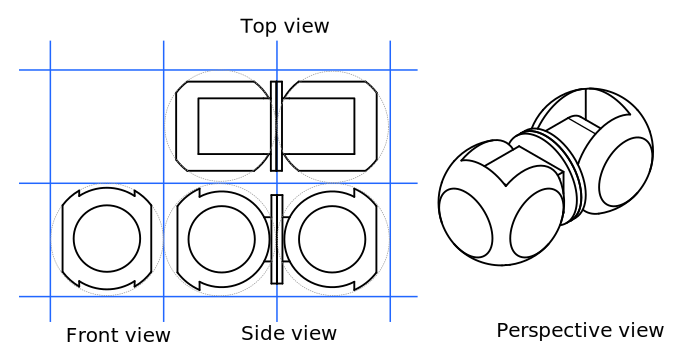
\includegraphics[width=\textwidth]{figures/rofi_reference.pdf}
    \caption{The universal RoFI module. Blue lines specify the grid, dotted
    lines marks spheres in which the module in inscribed. }
    \label{fig:rofi_reference}
\end{figure}

\begin{figure}
    \centering
    \includegraphics[width=0.7\textwidth]{figures/rofi_body_parts.pdf}
    \caption{Parts of the universal module.}
    \label{fig:rofi_body_parts}
\end{figure}

There are 3 degrees of freedom (figure \ref{fig:rofi_axis}):
\begin{enumerate*}
    \item shoe A can rotate against body A along the $\alpha$ axe in range
    $<-90^\circ; +90^\circ>$,
    \item shoe B can rorate against body B along the $\beta$ axe in range
    $<-90^\circ; +90^\circ>$ and
    \item body A can rotate against body B along the $\gamma$ axe in an
    unlimited range\footnote{First prototypes feature limitation on the $\gamma$
    axe due to technical limitations. }.
\end{enumerate*}
The module should be able to provide at least 1.5 $\text{N}\cdot\text{m}$ of
torque for each axe.

\begin{figure}
    \centering
    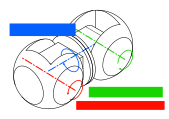
\includegraphics[width=0.7\textwidth]{figures/rofi_axis.pdf}
    \caption{Degrees of freedom of the universal module. The figure represents neutral position of each joint.}
    \label{fig:rofi_axis}
\end{figure}

The flat faces of shoes feature docking system for establishing mechanical
connection to other modules. There are 6 docks in total (figure
\ref{fig:rofi_locks}); 3 on each shoe. The docks are marked by the name of a
shoe and by one of following suffixes: -1, 0, 1. When facing the dock, its index
gives a factor by which we multiply degree of rotation to turn a shoe around its
axe in counter clockwise direction. Each dock is oriented. We denote the
orientation with an arrow. The dock orientation is important for describing
configurations of a system (more detail on that can be found in section
\ref{sec:configuration}). Details about docking mechanism are given in section
\ref{subsec:lock}.

\begin{figure}
    \centering
    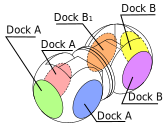
\includegraphics[width=0.7\textwidth]{figures/rofi_locks.pdf}
    \caption{Docks on the universal module. The arrow on each dock specifies its orientation.}
    \label{fig:rofi_locks}
\end{figure}

As it can be seen from the figures \ref{fig:rofi_reference} and
\ref{fig:rofi_body_parts}, the module does not occupy the whole space provided
by the grid. The module is (nearly) inscribed to two spheres (marked by a dotted
line in the figure \ref{fig:rofi_reference}). This allow the module to move its
shoe even if all neighbouring grid cells are occupied. We refer to this property
as \emph{grid-awareness}. This allows the module reconfigure more easily in
densely occupied grid -- see figure \ref{fig:grid_aware} for an example of such
a situation. Another perspective on grid-awareness of the universal module is
that no matter what position it is in, it never outreaches shape specified in
the figure \ref{fig:rofi_grid}.

\begin{figure}
    \centering
    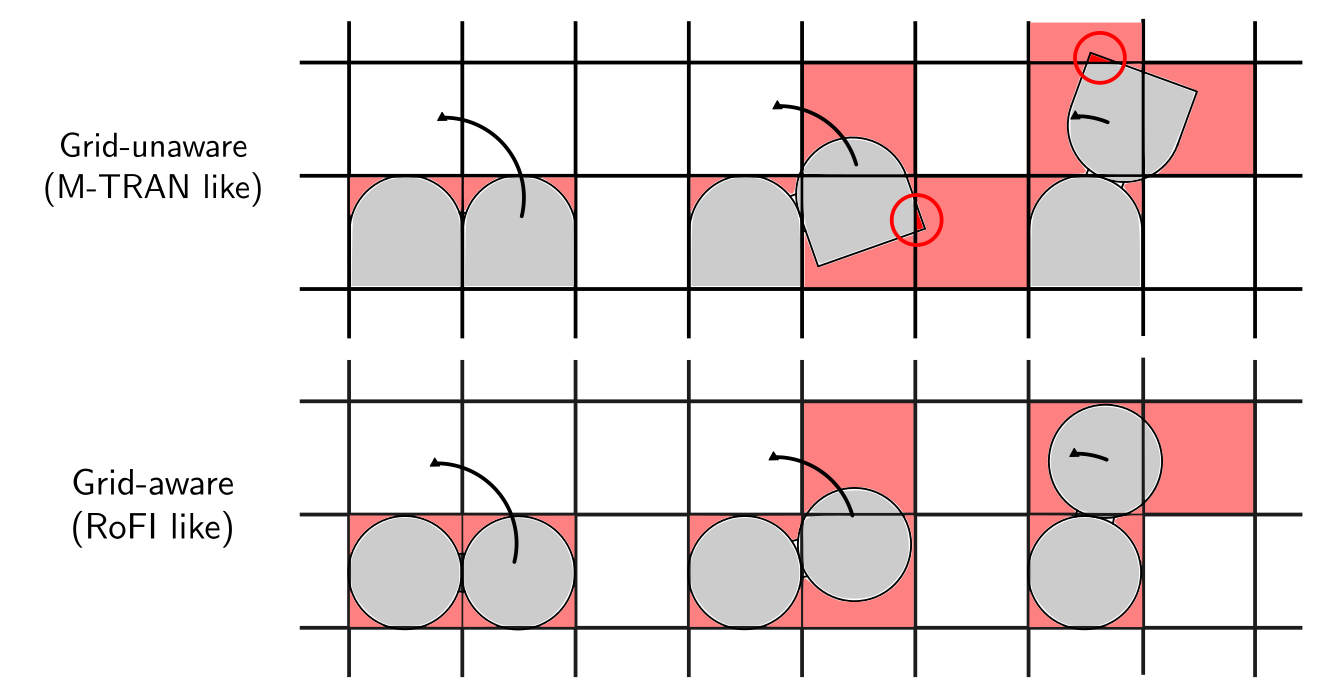
\includegraphics[width=\textwidth]{figures/grid_aware.pdf}
    \caption{Visualization of grid-awareness. Consider two module shapes -- M-TRAN\cite{haruhisa_kurokawa_m-tran_2003}
     like (int the top row) and RoFI like (in the bottom row). Given the task to
     move right body over the left one, M-TRAN like module occupies extra cells
     due to small parts of it body overlapping out of the gird. On the other
     hand, RoFI like module occupies the least cells required to make the
     movement.   }
    \label{fig:grid_aware}
\end{figure}

\begin{figure}
    \centering
    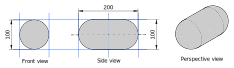
\includegraphics[width=\textwidth]{figures/rofi_grid.pdf}
    \caption{Reference shape for grid-awareness. If the module can be always inscribed in the shape, it is grid-aware.}
    \label{fig:rofi_grid}
\end{figure}

The grid-awareness prevents a face to face contact between two universal
modules. If the modules dock directly face to face, they would not fit in grid.
If the modules fully utilize the space allowed by the reference shape (figure
\ref{fig:rofi_grid}), they would feature only a point contact as two spheres
have only a single point touch. Therefore, there is a need for retractable
docking system. The docking system is specified in section \ref{subsec:lock}.
Here we only describe its relation to the grid.

If the module does not dock with another module, the dock is retracted in the
module shoe and therefore, the module does not outreach the reference shape.
When two modules dock to each other, the docks expand and connect to each other.
As the modules are now connected and no motion between them can be performed,
the enlarged footprint of module over the reference shape does not matter.
Illustration of the docking process can be found in the figure
\ref{fig:rofi_locking_example}.

\begin{figure}
    \centering
    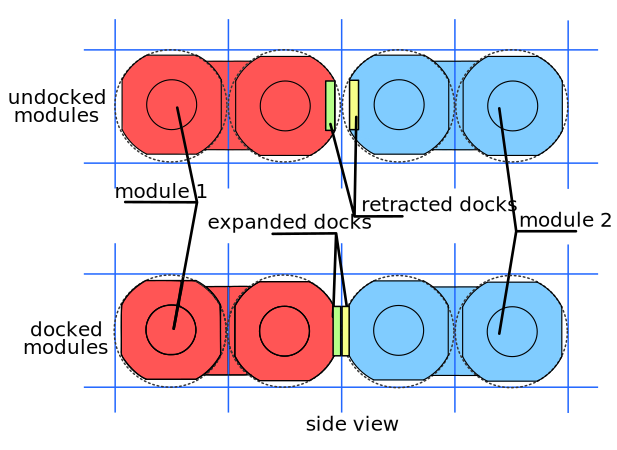
\includegraphics[width=\textwidth]{figures/rofi_locking_example.pdf}
    \caption{Docking procedure. There is a by-default retracted docking system
    in the module which expands when the docking should be performed.}
    \label{fig:rofi_locking_example}
\end{figure}

\subsection{Defining Custom Modules}\label{subsec:custom_modules}

\subsection{Docking System}\label{subsec:lock}

\subsection{RoFI Configuration and Capabilities} \label{sec:configuration}

To ease and unify the development of a firmware and reconfiguration algorithms,
we give means to describe the system made out of RoFI modules. First, there is
a globally unique ID (\emph{GUID}) assigned to each module. GUID is a 128-bit
number. Second, when talking about RoFI systems, we distinguish two terms:
\emph{topology} and \emph{configuration}: \todo{or configuration and realisation?}

\paragraph{topology} Intuitively, topology describes the connection between the
modules in a system and does not care about physical layout of the modules.
Formally, we define it as an undirected graph, where:
\begin{itemize}
    \item nodes are labeled by module GUIDs. There is exactly one node for each
    module in the system.
    \item edges represent a connection two docks. The edge is labeled by a pair
    describing the connection. For modules with GUIDs $a$ and $b$, connection by
    docks $d_a$ and $d_b$ in an orientation $o$ the label is: $(o, \{(a, d_a),
    (b, d_b)\})$. There is at most one edge for each dock on the module. The
    orientation of docks is defined further in the text. Note that undirected
    edges enforces that both modules has to actively participate on a
    connection.
\end{itemize}
\todo{Give an example (text + figure)}

\paragraph{configuration} Intuitively, configuration is a topology with the
actual module positions. Formally, it is a pair $(G, L)$, where $G$ is a
topology and $L: \text{GUID} \rightarrow \text{Axis} \rightarrow \mathcal{R}$ is
a function giving us position of each axis of each module.

As we mentioned in sections \ref{subsec:universal_module} and \ref{subsec:lock},
each dock features an orientation vector. When two docks connect, their
orientation vectors can hold angle of $0^\circ$, $90^\circ$, $180^\circ$ or
$270^\circ$ (measured counter clockwise from a perspective one of the modules
from shoe center to the dock center). Notice, that the angle is the same no
matter which module we choose. Therefore, we give a following convention for the
orientation:

If we aim one of the orientation vectors up (to the \emph{north}), the other
vector aims either:
\begin{enumerate*}
    \item \emph{north},
    \item \emph{east},
    \item \emph{south} or
    \item \emph{west}
\end{enumerate*}
as shown on figure \ref{fig:dock_orientation}.
Therefore we define the orientation $o$ to be an element of $O = \{N, E, S,
W\}$.

\begin{figure}
    \centering
    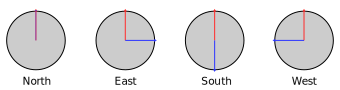
\includegraphics[width=\textwidth]{figures/dock_orientation.pdf}
    \caption{Possible orientation of two dock. Orientation vector of current
    perspective is shown as red, the orientation vector of mating dock is shown
    as blue. Note that it during a connection, it does not matter which dock's
    perspective we choose.}
    \label{fig:dock_orientation}
\end{figure}

We define \emph{model} of an configuration $(G, L)$ intuitively as a volumetric
body of a system of modules connected according to a topology $G$ with
axis oriented according to $L$ \todo{this is shady...}. We call a configuration
\emph{possible} iff a corresponding model exists (this can happen due to
inconsistency of axis orientation) and the model does not intersect itself.
\todo{Give example of possible configuration, impossible due to both factors}
Note, that there are no constraints on topology and we consider every topology
as valid. However, for some topologies there exists no possible configuration.

\subsection{Intermodule Communication and Power Sharing}

\subsection{Intramodule Architecture}

\subsection{The RoFI "BIOS" \todo{Proper naming}}

\subsection{RoFI lib}

\todo{Something here}

\todo{Define configuration somewhere}
\chapter{Universal Module}\label{chap:universal_module}

Chapter \ref{chap:rofi} gives the specification for modules in the RoFI
platform. In this chapter, we present the \emph{universal module}. This module
is supposed to be the primary building block of RoFI systems. It should provide
enough versatility to build a broad range of systems.

This chapter provides an overview of the design of the universal module and
gives a specification to implement it. The current state of implementation is
discussed in chapter \ref{chap:prototypes}.

\section{Universal Module Shape}

The universal RoFI module occupies two adjacent cells of the grid as can be seen
in figure \ref{fig:um_reference}. Please note that this drawing gives a
simplified model in which many technical details are omitted\footnote{You can
compare the simplified model with the physical prototype in chapter
\ref{chap:prototypes} -- the simplified model keeps the notion of the grid
spheres.}. The module arrangement is inspired by the M-TRAN
\cite{kurokawa_distributed_2008}. Unlike M-TRAN, the universal module is
grid-aware. The module composes of four parts:
\begin{enumerate*}
    \item \emph{body A},
    \item \emph{body B},
    \item \emph{shoe A}, and
    \item \emph{shoe B}.
\end{enumerate*}
-- see figure \ref{fig:um_body_parts}. Bodies are supposed to encapsulate
actuators, electronics, and accumulators; shoes are meant to provide connection
to other modules and provide movement.

\begin{figure}[t]
    \centering
    \includegraphics[width=\textwidth]{figures/um_reference.pdf}
    \caption{The universal RoFI module. The lines specify the grid, dotted
    lines marks spheres in which the module in inscribed. Note that we show the
    module with the Z axis facing right as it better fits the page layout. }
    \label{fig:um_reference}
\end{figure}

\begin{figure}[t]
    \centering
    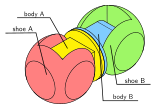
\includegraphics[width=0.7\textwidth]{figures/um_body_parts.pdf}
    \caption{Parts of the universal module.}
    \label{fig:um_body_parts}
\end{figure}

There are 3 degrees of freedom (figure \ref{fig:um_axis}):
\begin{enumerate}
    \item shoe A can rotate against body A along the $\alpha$ axis in a range
    $\langle -90^\circ; +90^\circ\rangle$,
    \item shoe B can rotate against body B along the $\beta$ axis in a range
    $\langle -90^\circ; +90^\circ\rangle$, and
    \item body A can rotate against body B along the $\gamma$ axis in $\langle
    -180^\circ; +180^\circ\rangle$ with an overflow\footnote{First prototypes
    feature a limitation on a number of overflows in one direction on the
    $\gamma$ axis due to technical limitations. }.
\end{enumerate}
The module should be able to provide at least 1.5 $\text{N}\cdot\text{m}$ of
torque for each axis.

\begin{figure}[!t]
    \centering
    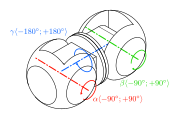
\includegraphics[width=0.7\textwidth]{figures/um_axis.pdf}
    \caption{Degrees of freedom of the universal module. The figure represents
    neutral position of each joint.}
    \label{fig:um_axis}
\end{figure}

There are 3 docks on each shoe -- dock $X+, X-$ and $Z-$. The position of the
docks is captured in figure \ref{fig:um_docks}. The shape descriptor in figure
\ref{fig:um_descriptor} captures the universal module arrangement.

\begin{figure}[!t]
    \centering
    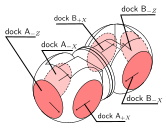
\includegraphics[width=0.7\textwidth]{figures/um_docks.pdf}
    \caption{Docks on the universal module. The arrow on each dock specifies its orientation.}
    \label{fig:um_docks}
\end{figure}

Such module arrangement is more versatile than the M-TRAN arrangement. Addition
of the third axis, the $\gamma$ axis, overcomes two limitations of M-TRAN-like
arrangement:
\begin{enumerate*}
    \item given a chain configuration with all joints parallel to each other,
    the system can span only in two dimensions; it cannot expand into the third
    dimension.
    \item Also, given a roller configuration (figure \ref{fig:example_roller})
    which can roll forward, the M-TRAN module cannot steer and only moves
    forward.
\end{enumerate*}

\begin{figure}[!t]
    \centering
    \begin{subfigure}[b]{0.45\textwidth}
        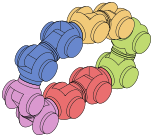
\includegraphics[width=\textwidth]{figures/ring_example.pdf}
        \caption{Roller}
        \label{fig:example_roller}
    \end{subfigure}
    ~
    \begin{subfigure}[b]{0.45\textwidth}
        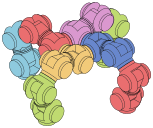
\includegraphics[width=\textwidth]{figures/spider_example.pdf}
        \caption{Spider}
        \label{fig:example_spider}
    \end{subfigure}

    \caption{Examples of RoFI systems.}
    \label{fig:examples}
\end{figure}

\section{Universal Module Sensors}

We design the universal module to be rather sensor-impecunious rather than
sensor-rich. We suppose there will be various RoFI systems with various
sensor needs. Therefore, we find much useful to implement in the universal
module only sensors that can be beneficial nearly in all systems. The special
sensors for concrete systems should be implemented as separate modules.

There are two types of sensors in each universal module:
\begin{enumerate*}
    \item inertial measurement unit (IMU) and
    \item distance sensors in the middle of each dock.
\end{enumerate*}
The IMU provides a basic notion of the module orientation in the space. Data
from IMU can be used in algorithms to, e.g., determine a common direction in
space among all modules using the Earth's gravitational force. A good solution
for the IMU IC is MPU-9250 \cite{noauthor_mpu-9250_2016} due to broad community
support and all-in-one-package solution (accelerometer, gyroscope, and
magnetometer).

We plan to use the VL53L1X \cite{noauthor_new_2018} time-of-flight distance
sensor in each dock. The sensors allow the universal module to detect obstacles
in front of the module, help to establish correct alignment of two docks when
connecting and can also be used to scan the environment. The scanning of the
environment is performed by moving a shoe and building a depth map. The depth
map can be used as a simple input for computer vision. For example, when a RoFI
system is supposed to climb stairs, it can measure their geometry by this
procedure.

\section{Intra-module Architecture}

Each universal module is an autonomous unit. A single \emph{control unit}
controls the module. This unit controls all the other components of the module
as can be seen in figure \ref{fig:um_internal}. The unit controls smart
servomotors over a bus built on top UART, docks over SPI bus and directly
controls charging and power management circuits.

\begin{figure}[!t]
    \centering
    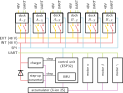
\includegraphics[]{figures/um_internal.pdf}
    \caption{Block diagram of internal architecture of the module.}
    \label{fig:um_internal}
\end{figure}

\subsection{Control Unit}

The control unit is designed to be powered by the ESP32 microcontroller
\cite{noauthor_esp32_2018}. This microcontroller provides enough computational
power, provides rich peripherals including Bluetooth 4 Low Energy and WiFi
802.11 b/g/n, and most importantly, the vendor provides excellent software
support. We are mainly concerned by three aspects of the software support:
\begin{enumerate*}
    \item there is support for modern C/C++ compilers with full support for the
    C++ standard library (including exception handling and concurrency),
    \item the development framework provides POSIX compatible interface, and
    \item there is a vendor maintained port of the lwIP library.
\end{enumerate*}

First two aspects are crucial for easy development of software. From a practical
aspect, the ESP32 is nearly indistinguishable from a desktop POSIX environment
while it still preserves real-time nature and easy access to low-level
peripherals. The POSIX compatibility allow the developers to leverage existing
libraries and port them to the universal module without a significant effort.
The support for lwIP is a benefit as the control unit serves as network
switch (as defined in section \ref{sec:communication}) and therefore, we can
use it. The only necessary part of implementing is the custom device driver for the
docks.

The control unit is not supposed to provide any sensors except the IMU since the
placement of IMU in the robot is not crucial. The distance sensors on the docks
are controlled by a microcontroller on the dock and the control unit.


\subsection{Motors}

We decided to use so-called \emph{smart servomotors} (servos) to power the
universal module. These servos are similar to their hobby counterparts. Just
like the hobby servo, a smart servo is a DC motor with a gearbox combined with a
driver and feedback loop controller in a single compact package. The main
difference between these two is that smart servos provide a digital bus for
sending commands (unlike pulse-width modulation communication used in hobby
servos) and offer several advanced features. The hobby servo can be controlled
only in position mode without any feedback to the control system. The smart
servos usually allow for multiple control modes (torque, speed, and position),
allow continuous rotation and also provide feedback to the control system.
Therefore, the system can detect when the motor reaches a commanded
position or if the motor is overloaded.

The usage of smart servos simplifies both, the mechanical construction and the
control unit, as we can omit motor driver, custom gearing and encoders. In our
design, we use HerkuleX DRS-0101 \cite{noauthor_herkulex_nodate} servos. These
servos are designed to be powered directly from a two cell li-ion accumulator
and provide 1.2 N$\cdot$m of torque at maximal speed one turn per second. The
servos communicate over UART bus, where the control unit serves as a master and
the servos are slaves. The servos can be daisy-chained and therefore, only two
wires are required for the communication. The command set provides means to
perform a synchronized movement.

We choose the DRS-0101 servos for several reasons: they feature slightly smaller
mechanical size compared to the Dynamixel AX-12A \cite{noauthor_dynamixel_2006}
(a comparable servo), they are mechanically compatible with DRS-0201
\cite{noauthor_herkulex_nodate} servos, which feature twice the power. The servo
is also mechanically compatible with Lewansoul LX-16A
\cite{noauthor_lx-16a_2018}, which is a low-cost alternative for possible future
mass production.

\subsection{Power Management}

The module is supposed to be powered from a two cell li-ion accumulator pack.
The motors can directly operate from the accumulator at their rated voltage and
can drain sufficient current. The control unit is also powered from the
accumulator.

The internal connection of power rails is captured in figure
\ref{fig:um_internal}. There is a charger circuit to allow for charging from the
INT line. The charger is controlled by the control unit -- it can be either
disabled or it can charge the accumulator with given power limit. There is also
a step-up convertor used to source power to other modules. The used step-up
convertors must be parallelizable (denoted by a diode in the block diagram). The
step-up module is also controlled by the control unit and can be disabled when
not needed. Having this power sharing setup, the module can operate in four
modes:

\paragraph{Self-powered mode} The module runs on its own accumulator (charger is
disabled and convertor is disabled).

\paragraph{Power sourcing mode} The module provides energy to the network
(charger is disabled and convertor is enabled).

\paragraph{Power draining mode} The module charges its accumulator and drains
power from other modules.

\paragraph{Survivor mode} The module disables motors, disables converter and
limits the charging power roughly to cover energy consumption of the control
module. Therefore, no charging occurs and the charger is acts as a step-down
converter for the control unit.

The communication in the RoFI platform requires an activity from the control
unit as it routes packets between the docks. If a module shuts down due to
discharged accumulator, there cannot be any communication across the module.
Dead module might lead to a separation of the system into two independent
networks in some configurations. Therefore, survivor mode can be applied to keep
the communication going without waisting power on charging the dead module.

\chapter{Behind the RoFI design}\label{chap:behind}

\todo{Something here}
\chapter{The RoFI Prototypes}\label{chap:prototypes}

The RoFI project as defined in the previous chapter is broad and, therefore,
implementing all of the proposed solutions in the full depth is far beyond the
reach of the thesis. Therefore, we focused on three the most important aspects
of the RoFI project. We would like to show that:
\begin{itemize}
    \item the docking mechanism can be built and that it features claimed
    properties,
    \item integration of TCP/IP communication in the system using a custom
    hardware layer is possible; and
    \item the universal module can be built.
\end{itemize}
All the source codes and CAD models of results presented here can be found in a
Git repository \url{https://github.com/paradise-fi/RoFi}.

\section{Docking Mechanism}

\section{Inter-module Communication}

We proposed in section \ref{sec:communication} that the modules in a RoFI system
should communicate using a TCP/IP networking as it allows to easily adapt
existing algorithms and technical solutions. The proposed solution implements a
custom layer two of the standard ISO/OSI model.

To show the feasibility of the proposed solution, we have implemented a simple
prototype. The prototype does not provide any mechanical hardware, it consists
only of several interconnected development modules with microcontrollers. We
implemented a firmware for the ATMega328p microcontroller providing the dock
protocol (section \ref{sec:dock_interface}) and a corresponding part of the RoFI
driver for the ESP32 microcontroller -- dock driver, address mapping protocol
and interface for the lwIP TCP/IP stack. Both implementation can be found in the
project repository.

The ATMega328p was chosen due availability of cheap development modules in form
Arduino Nano and low-effort development. This decision allowed us to quickly get
a working prototype, however, at the cost of not providing solution with low
performance as we reached memory and computational limits of the
microcontroller. The limitations come in form of limited SPI clock speed
(100~kHz) and smaller maximal blob size (128 bytes). We consider the
implementation of the firmware straightforward and not worth further
description.

On the other hand, the implementation of the RoFI driver for ESP32 we provide is
intended for future use. The driver is written in C++14. It is structured in two
classes: \texttt{Dock} (direct interface for a single dock) and \texttt{Roif}
(network interface built on top docks).

\texttt{Dock} automatically handles communication with the docks, i.e., hides
all details of the communication (e.g., interrupt handling) and provides a
simple interface: user can supply a binary blob (in form of the \texttt{pbuf}
structure from lwIP) or be notified with an incoming blob via a callback. The
interface for changing or querying dock state (retracting or expanding of the
dock, querying the state of the power lines, etc.) is implemented in similar
fashion. Our implementation prevents congestion of the shared SPI bus by
limiting the number of pending queries per dock and therefore, allowing for fair
usage of the bus.

The challenge of the implementation was mapping SPI transaction to the interface
provided by ESP32 development framework (ESP-IDF). ESP-IDF provides a way to
queue asynchronous SPI transactions with distinct read and write phases
including delay between the phases. However, it does not support transactions
with variable length, which are required by our protocol. The transactions have
to be implemented using several SPI transaction offered by ESP-IDF. The naive
implementation is not possible as transactions from multiple docks could
interleave and therefore, yield incorrect results. There are two possible
approaches to tackle this problem: we can either queue transactions in advance
and modify them on the fly, or we can use a separate FreeRTOS task executing
blocking SPI transactions. Our implementation uses the second solution as our
analysis of the ESP-IDF source code shows that changing already queued
transactions is not safe and also, the first solution requires non-trivial
locking. The second solution also produces easier to follow code with no
explicit locking as all the locking is handled by FreeRTOS and therefore, was
chosen.

\texttt{Roif} (\emph{Ro}Fi network \emph{in}terface) provides a glue between
docks and lwIP. It handles registration of a new network interface and all the
required callbacks (as we mentioned in section \ref{sec:networking}). It also
features implementation of the address mapping protocol to determine which dock
should be used for outgoing communication.

As a by-product of the implementation of the RoFI driver, we implemented set of
C++ wrappers for the FreeRTOS API. Unlike the already existing C++ wrappers we
are aware of, we do not simply rename functions and group them in classes like
these wrappers. Our wrappers respect C++ idioms and also provide proper C++ copy
and move semantics. Such wrapper allows the user to write easier to understand
and less error-prone code. At the time of writing this theses, the FreeRTOS
wrapper was not separated into a stand-alone project.

\begin{figure}[!t]
    \centering
    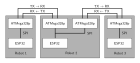
\includegraphics[width=\textwidth]{figures/communication_setup.pdf}
    \caption{The setup for our inter-module communication prototype.}
    \label{fig:comm_setup}
\end{figure}

We tested our implementation in a simple setup shown at figure
\ref{fig:comm_setup}. We used three ESP32-DevkitCs simulating module
controllers, and for Arduino Nanos simulating the docks. We wired them as shown
in the figure. Then, we were able to successfully establish both, TCP and UDP,
connections. The codes for establishing the connections are a simple example
inspired by official demo codes. There are no modification for our setup. The
example codes can be found in the project repository.

Replication of our results should be fairly straightforward as we ship all the
code as PlatformIO\footnote{\url{https://platformio.org/}} projects, therefore
no complicated toolchain setup is necessary; and also, the hardware we use is
commonly available.However, during testing of our firmware we encountered a bug
in lwIP implementation preventing a TCP connection from being opened. The bug
has been already fixed in the lwIP upstream repository, however at the time of
writing this thesis, the lwIP library shipped with ESP-IDF was not updated.
Therefore, to successfully run the TCP example, manual update of the library is
necessary.

\section{Universal Module}



\chapter*{Bibliography}
\addcontentsline{toc}{chapter}{Bibliography}
\markboth{}{} % avoid headers from last chapter in bibliography
\printbibliography[heading=none]

\appendix
\chapter{TBA}

\end{document}